\chapter{Financial Assessment}
In this part an analysis of the economic performances of the service proposals is presented. The analysis follows the two scenarios:
•	A: characterized by the implementation of new rides from scratch;
•	B: defined by modification of the actual lines.
The objective of this part is to access the scenario that, a parity of level of service for the customer and general assumptions, is the most financially profitable and sustainable.
The initial part regarding the Fare Revenues analysis is common for both the scenario. Instead, the economic performance of the two scenarios will be studied separately.


\paragraph{Economic Analysis assumptions}
The provided assumption used to perform this analysis are reported for reference in the table \ref{tab:specificcostbus} and regards the specific cost of a bus service. 

% Please add the following required packages to your document preamble:
% \usepackage[table,xcdraw]{xcolor}
% If you use beamer only pass "xcolor=table" option, i.e. \documentclass[xcolor=table]{beamer}
% \usepackage{lscape}

\begin{table}[H]
\centering
\begin{tabular}{lll}
\hline
\rowcolor{bluepoli!40}
\multicolumn{1}{|c|}{{\color[HTML]{333333} \textbf{Bus operation related cost}}} & \multicolumn{1}{c|}{{\color[HTML]{333333} \textbf{Local   currency}}} & \multicolumn{1}{c|}{{\color[HTML]{333333} \textbf{12   m bus}}} \\ \hline
\multicolumn{1}{|l|}{{\color[HTML]{333333} Fuel price}}                          & \multicolumn{1}{l|}{{\color[HTML]{333333} €/Litre}}                   & \multicolumn{1}{l|}{{\color[HTML]{333333} 1.20}}                \\ \hline
\multicolumn{1}{|l|}{{\color[HTML]{333333} Fuel Consumption}}                    & \multicolumn{1}{l|}{{\color[HTML]{333333} Km/Litre}}                  & \multicolumn{1}{l|}{{\color[HTML]{333333} 2.50}}                \\ \hline
\multicolumn{1}{|l|}{{\color[HTML]{333333} Maintenance cost per year}}           & \multicolumn{1}{l|}{{\color[HTML]{333333} €/Km}}                      & \multicolumn{1}{l|}{{\color[HTML]{333333} 0.25}}                \\ \hline
\multicolumn{1}{|l|}{{\color[HTML]{333333} Mileage per year}}                    & \multicolumn{1}{l|}{{\color[HTML]{333333} Km}}                        & \multicolumn{1}{l|}{{\color[HTML]{333333} 50,000}}              \\ \hline
\multicolumn{1}{|l|}{{\color[HTML]{333333} Capital expenditure per bus}}         & \multicolumn{1}{l|}{{\color[HTML]{333333} €}}                         & \multicolumn{1}{l|}{{\color[HTML]{333333} 200,000}}             \\ \hline
\multicolumn{1}{|l|}{{\color[HTML]{333333} Years in operation}}                  & \multicolumn{1}{l|}{{\color[HTML]{333333} \#}}                        & \multicolumn{1}{l|}{{\color[HTML]{333333} 15}}                  \\ \hline
\multicolumn{1}{|l|}{{\color[HTML]{333333} Amortization index}}                  & \multicolumn{1}{l|}{{\color[HTML]{333333} \#}}                        & \multicolumn{1}{l|}{{\color[HTML]{333333} 6.7\%}}               \\ \hline
{\color[HTML]{333333} }                                                          & {\color[HTML]{333333} }                                               & {\color[HTML]{333333} }                                         \\ \hline
\rowcolor{bluepoli!40}\multicolumn{1}{|c|}{{\color[HTML]{333333} \textbf{Other Costs}}}                & \multicolumn{1}{c|}{{\color[HTML]{333333} \textbf{Local   currency}}} & \multicolumn{1}{l|}{{\color[HTML]{333333} }}                    \\ \hline
\multicolumn{1}{|l|}{{\color[HTML]{333333} Driver cost per year STD}}            & \multicolumn{1}{l|}{{\color[HTML]{333333} €}}                         & \multicolumn{1}{l|}{{\color[HTML]{333333} 35,000}}              \\ \hline
\multicolumn{1}{|l|}{{\color[HTML]{333333} workdays}}                            & \multicolumn{1}{l|}{{\color[HTML]{333333} }}                          & \multicolumn{1}{l|}{{\color[HTML]{333333} 250}}                 \\ \hline
\multicolumn{1}{|l|}{{\color[HTML]{333333} hours per year STD}}                  & \multicolumn{1}{l|}{{\color[HTML]{333333} }}                          & \multicolumn{1}{l|}{{\color[HTML]{333333} 1,800}}               \\ \hline
\multicolumn{1}{|l|}{{\color[HTML]{333333} Insurance per bus}}                   & \multicolumn{1}{l|}{{\color[HTML]{333333} €/bus}}                     & \multicolumn{1}{l|}{{\color[HTML]{333333} 2,000}}               \\ \hline
\multicolumn{1}{|l|}{{\color[HTML]{333333} Selling expenses}}                    & \multicolumn{1}{l|}{{\color[HTML]{333333} }}                          & \multicolumn{1}{l|}{{\color[HTML]{333333} 2\%}}                 \\ \hline
\multicolumn{1}{|l|}{{\color[HTML]{333333} Annual budget marketing expenses}}    & \multicolumn{1}{l|}{{\color[HTML]{333333} }}                          & \multicolumn{1}{l|}{{\color[HTML]{333333} 10,000}}              \\ \hline
\multicolumn{1}{|l|}{{\color[HTML]{333333} Tax}}                                 & \multicolumn{1}{l|}{{\color[HTML]{333333} }}                          & \multicolumn{1}{l|}{{\color[HTML]{333333} 27.9\%}}              \\ \hline
\end{tabular}
\caption{Specific cost of a Bus Service}
\label{tab:specificcostbus}
\end{table}% tabella


\section{Fare revenues}
To select the cost, a weighted average between the distance of the proposed service has been made: a weight of 80\% has been added to category 8 (to address the amount of workers arriving from Voghera); a weight of 20\% to category 3 (to address the workers arriving from Stradella and Broni). So, the resultant ticket category is 7.

The starting point of the fare revenue analyses has been the definition of its value on monthly base by the income from travel documents sale. This value is strongly correlated not simply with the number of tickets sold, but even more by the typology of the document due to the subscription discount factor.
\begin{table}[H]
\centering
\begin{tabular}{|l|l|l|l|l|}
\hline
\rowcolor{bluepoli!40}
\multicolumn{1}{|c|}{\textbf{\begin{tabular}[c]{@{}c@{}}Travel \\ Document \\ Typology\end{tabular}}} & \multicolumn{1}{c|}{\textbf{Cost}} & \multicolumn{1}{c|}{\textbf{\begin{tabular}[c]{@{}c@{}}\# journey \\ per ticket\end{tabular}}} & \multicolumn{1}{c|}{\textbf{\begin{tabular}[c]{@{}c@{}}Cost \\ of \\ single travel\end{tabular}}} & \multicolumn{1}{c|}{\textbf{\begin{tabular}[c]{@{}c@{}}Discount \\ factor\end{tabular}}} \\ \hline
Single ticket                                                                                         & 3.7                                & 1                                                                                              & 3.70                                                                                              & 0\%                                                                                      \\ \hline
10 Journey ticket                                                                                     & 34.5                               & 10                                                                                             & 3.45                                                                                              & 7\%                                                                                      \\ \hline
Weekly ticket                                                                                         & 24.5                               & 12                                                                                             & 2.04                                                                                              & 45\%                                                                                     \\ \hline
Monthly ticket                                                                                        & 86                                 & 48                                                                                             & 1.79                                                                                              & 52\%                                                                                     \\ \hline
Annual ticket                                                                                         & 830                                & 528                                                                                            & 1.57                                                                                              & 58\%                                                                                     \\ \hline
\end{tabular}
\caption{Tickets cost}
\label{tab:ticket}
\end{table}%tabella

In the following step, a possible composition of the travel documentation type is estimated. The first strong conceptual division of the analysis has been the differentiation between a high demand service and low demand ones, which is reflected into the general travel documentation typology composition.

\begin{figure}[h]
    \centering
    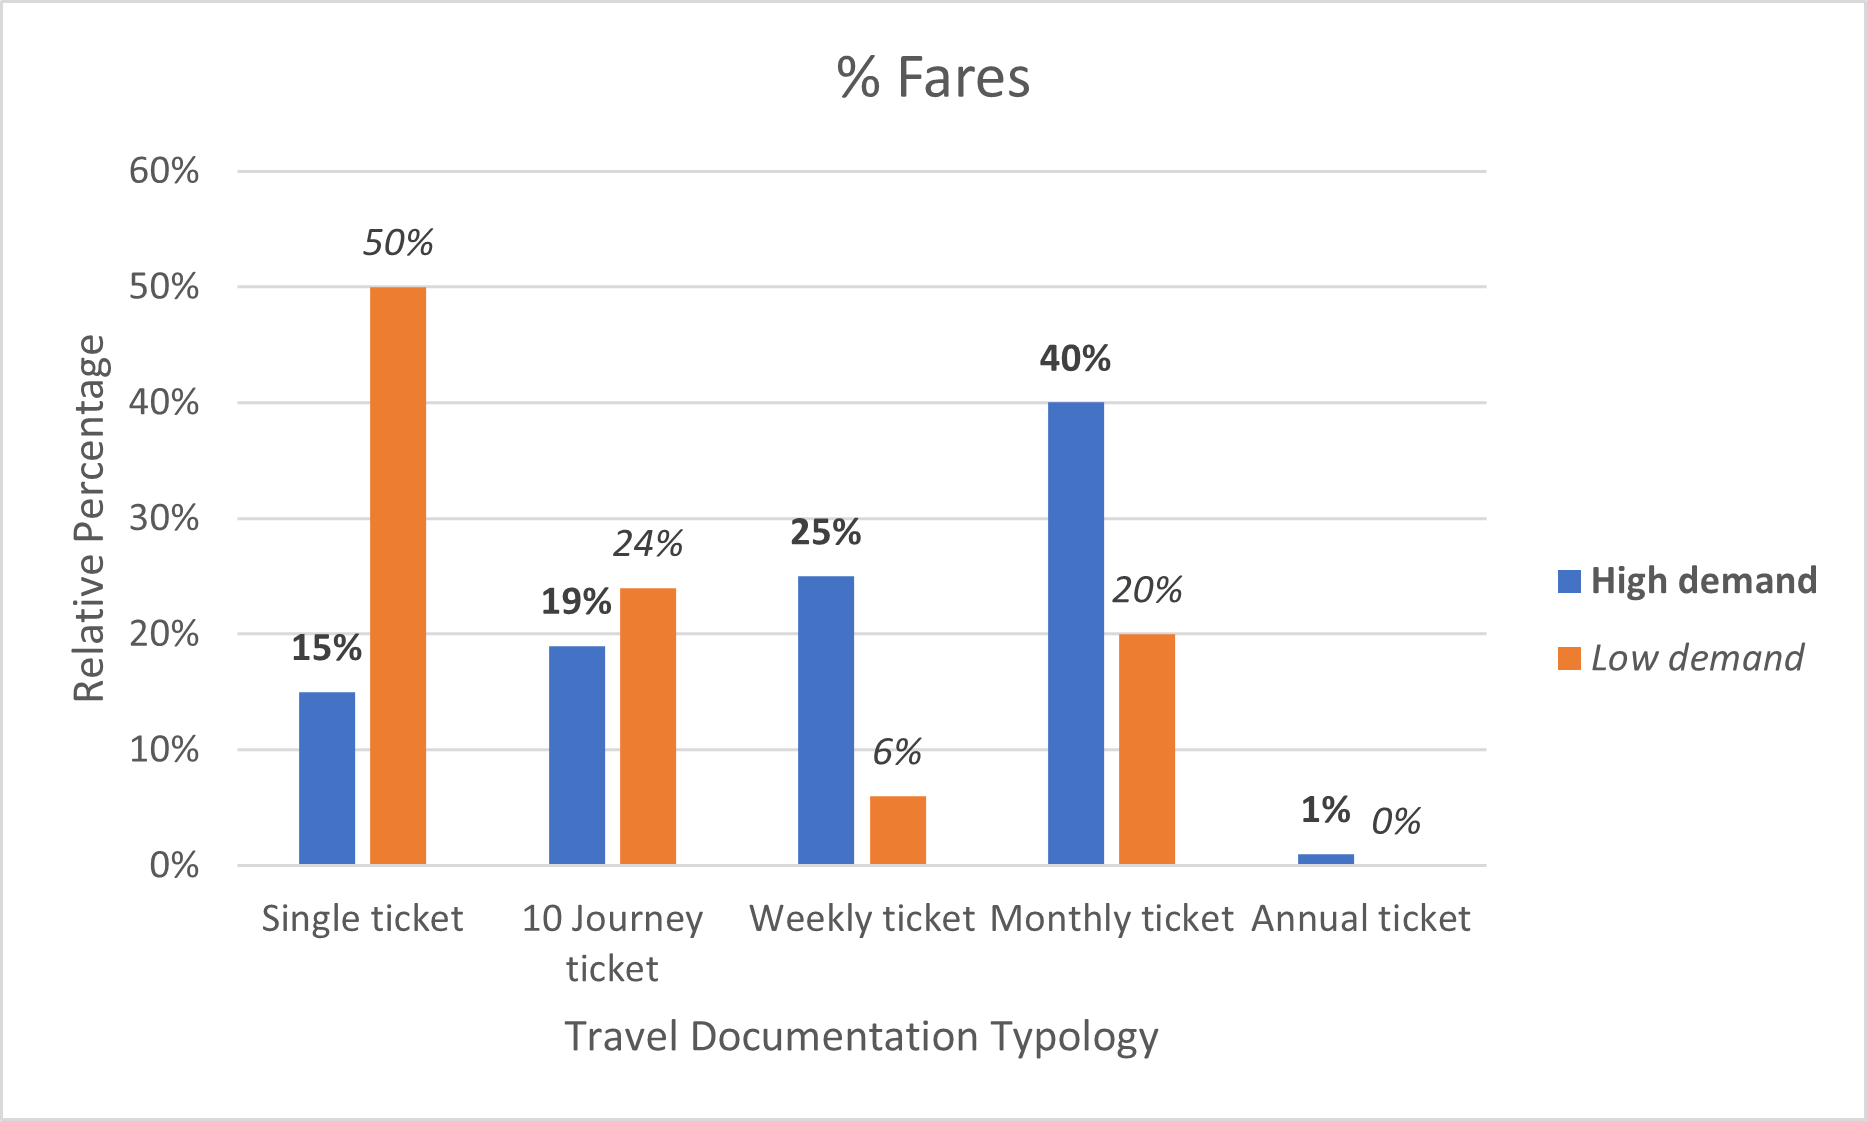
\includegraphics[width=0.7\textwidth]{Images/financial/fares.png}
    \caption{Fares percentage}
    \label{fig:fares_percentage}
\end{figure}
Considering the nature of the service under study, characterized by stable and a priori known demand, it can be easily clustered under the “High demand” service typology. This baseline feature is reflected in a travel documentation mix more oriented to subscription than single tickets.

The table \ref{tab:fare_distribution} and figure \ref{fig:fares_percentage2} represent the estimation of the travel documentation mix on the yearly base. This exercise has been performed to understand how the winter and summer working holiday period could be reflected in the customer choice.
\begin{figure}[h]
    \centering
    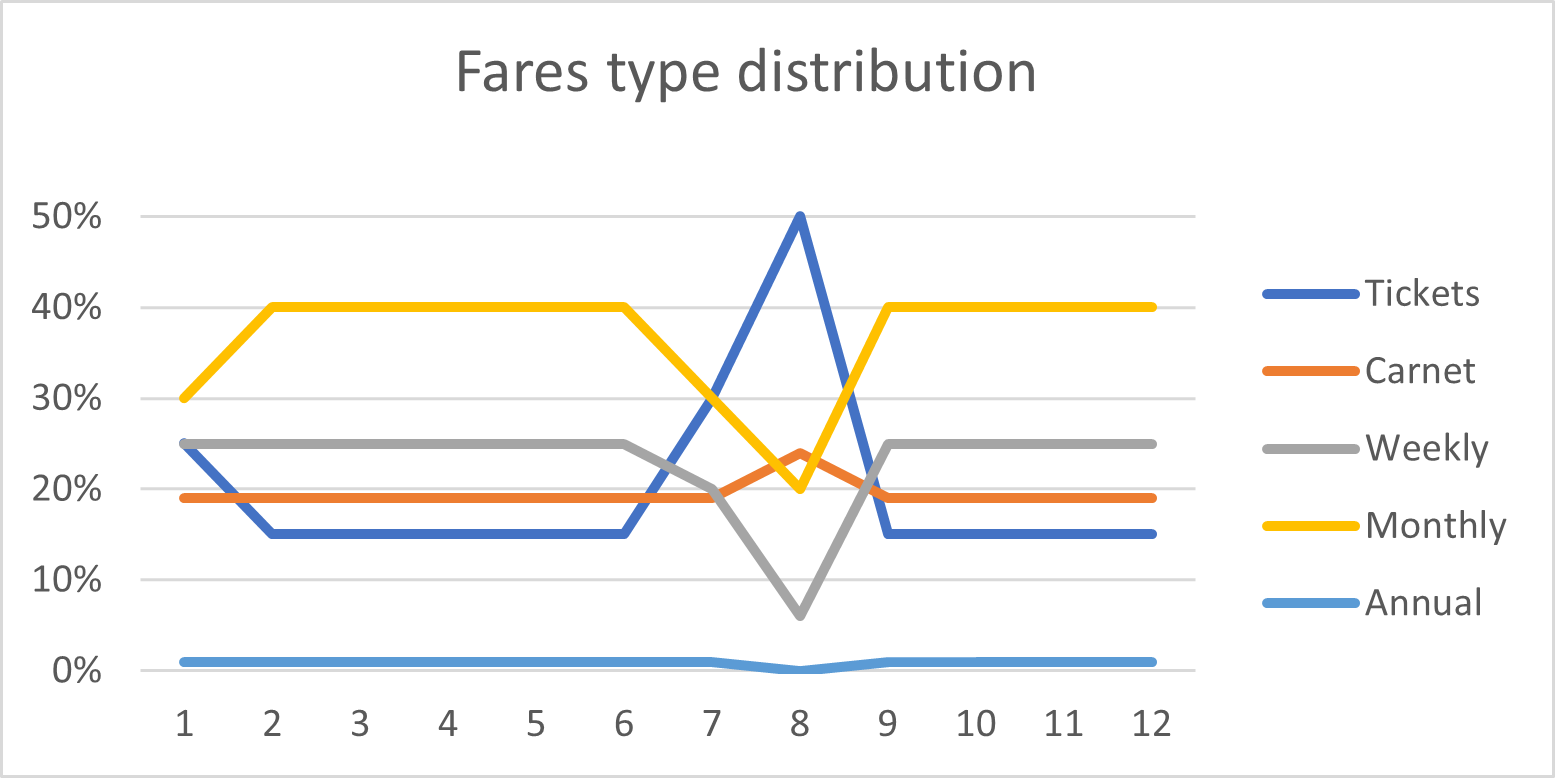
\includegraphics[width=0.7\textwidth]{Images/financial/fares_type_distribution.png}
    \caption{Fares percentage}
    \label{fig:fares_percentage2}
\end{figure}

% Please add the following required packages to your document preamble:
% \usepackage{multirow}
% \usepackage[table,xcdraw]{xcolor}
% If you use beamer only pass "xcolor=table" option, i.e. \documentclass[xcolor=table]{beamer}
\begin{table}[hp]
\centering
\begin{tabular}{|l|l|l|l|l|l|l|l|}
\hline
\rowcolor{bluepoli!40}
\multicolumn{1}{|c|}{\textbf{\begin{tabular}[c]{@{}c@{}}travel\\ documents\end{tabular}}} & \multicolumn{1}{c|}{{\color[HTML]{333333} \textbf{Year 1}}} & \multicolumn{1}{c|}{{\color[HTML]{333333} \textbf{Year 2}}} & \multicolumn{1}{c|}{{\color[HTML]{333333} \textbf{Year 3}}} & \multicolumn{1}{c|}{{\color[HTML]{333333} \textbf{Year 4}}} & \multicolumn{1}{c|}{{\color[HTML]{333333} \textbf{Year 5}}} & \multicolumn{1}{c|}{{\color[HTML]{333333} \textbf{Year 6}}} & \multicolumn{1}{c|}{\textbf{\begin{tabular}[c]{@{}c@{}}Yearly \\ variation {[}\%{]}\end{tabular}}} \\ \hline
Single ticket                                                                             & 19,584                                                      & 18,996                                                      & 18,427                                                      & 17,874                                                      & 17,338                                                      & 16,817                                                      & $-3\%$                                                                                             \\ \hline
10 Journey ticket                                                                         & 1,901                                                       & 1,863                                                       & 1,826                                                       & 1,789                                                       & 1,754                                                       & 1,719                                                       & $-2\%$                                                                                             \\ \hline
Weekly ticket                                                                             & 2,252                                                       & 2,253                                                       & 2,255                                                       & 2,256                                                       & 2,257                                                       & 2,258                                                       & $0\%$                                                                                              \\ \hline
Monthly ticket                                                                            & 898                                                         & 916                                                         & 934                                                         & 953                                                         & 972                                                         & 991                                                         & $2\%$                                                                                              \\ \hline
Annual ticket                                                                             & 22                                                          & 23                                                          & 23                                                          & 23                                                          & 23                                                          & 24                                                          & $1\%$                                                                                              \\ \hline
Annual journey                                                                            & 120,556                                                     & 120,583                                                     & 120,653                                                     & 120,766                                                     & 120,922                                                     & 121,120                                                     &                                                                                                    \\ \cline{1-7}
\begin{tabular}[c]{@{}l@{}}Fare \\ Reneues {[}€{]}\end{tabular}                           & 289,052                                                     & 287,326                                                     & 285,724                                                     & 284,243                                                     & 282,882                                                     & 281,639                                                     &                                                                                                    \\ \cline{1-7}
\begin{tabular}[c]{@{}l@{}}Fare \\ Reneues \\ variation {[}\%{]}\end{tabular}             & $0.0\%$                                                     & -0.6\%                                                      & $-1.2\%$                                                    & $-1.7\%$                                                    & $-2.1\%$                                                    & $-2.6\%$                                                    & \multirow{-3}{*}{}                                                                                 \\ \hline
\end{tabular}
\caption{Fare distribution output   }
\label{tab:fare_distribution}
\end{table}
Moving to the economical results of this travel documentation distribution mix, it is possible observing that the monthly ticket, that is around the 40\% of the total, generates the 60\% of the income.

\begin{figure}[h]
    \centering
    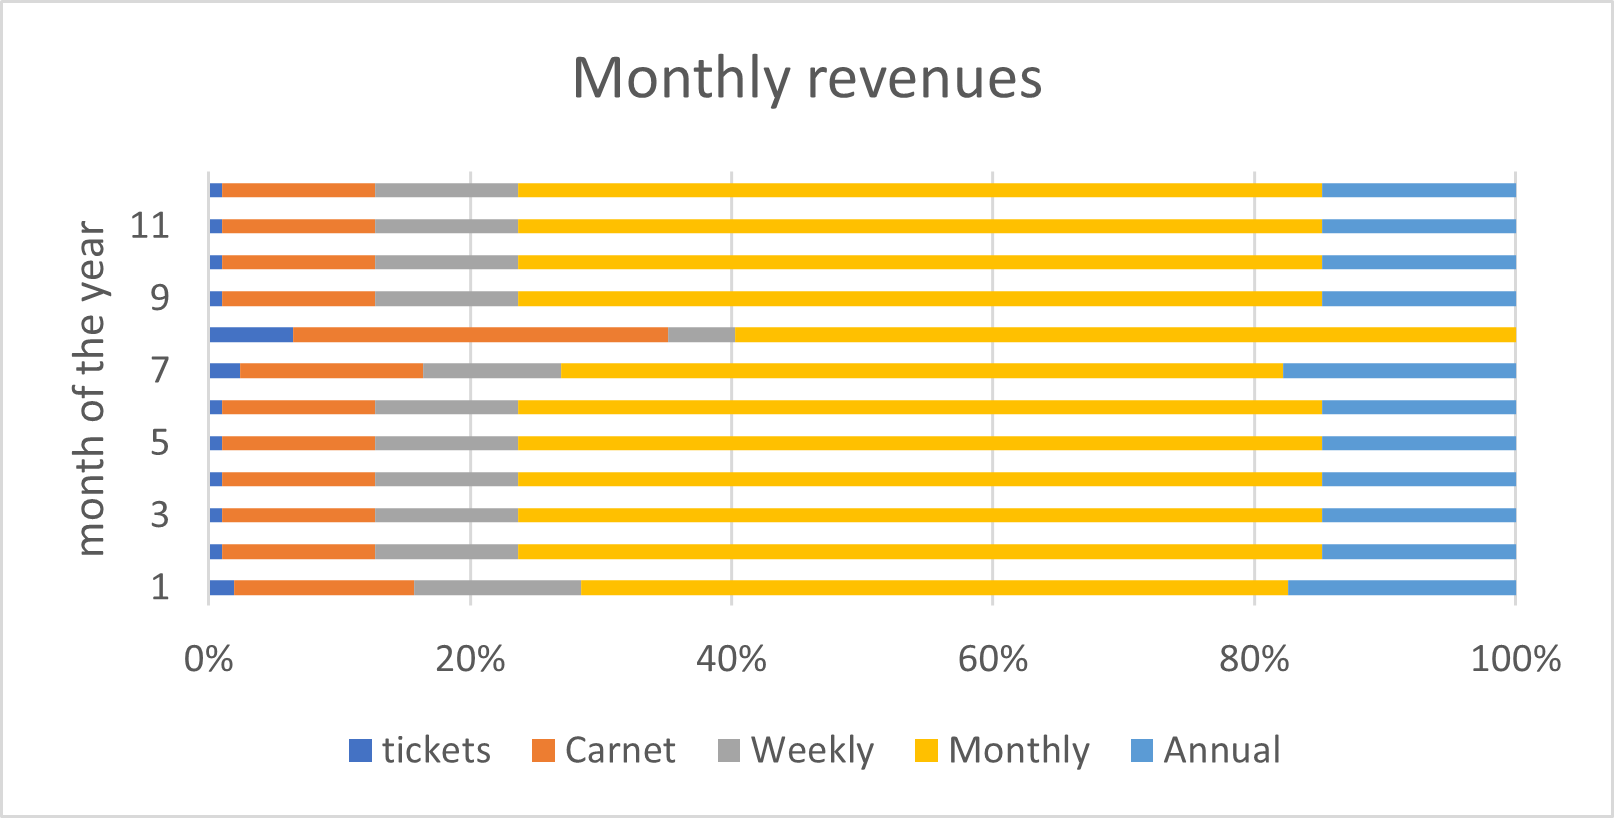
\includegraphics[width=0.7\textwidth]{Images/financial/monthly_revenues.png}
    \caption{Montlhy Revenues}
    \label{fig:monthly_revenues}
\end{figure}
To simulate the evolution of the customer behavior over the years under the “customer loyalty” concept, a progressive shift of the “ \% fares” from the short-term ticket type to the longer-term subscription is assumed and reported in the resuming table below.

Looking to the fare revenues results, the variation in the customer choice trend over the years leads to a constant erosion of the income due to the lower marginal value of the subscriptions. 

Given the positive financial results throughout the periods -showed in the following section-, this is not a negative phenomenon given the temporal profile nature of the subscription – comparable to a free interest tax loan – with respect to the single ticket ones. 

Finally, the figure \ref{fig:j_revenues} shows the relationship between journey performed, generated revenues and the ratio between ticket/subscription.

\begin{figure}[h]
    \centering
    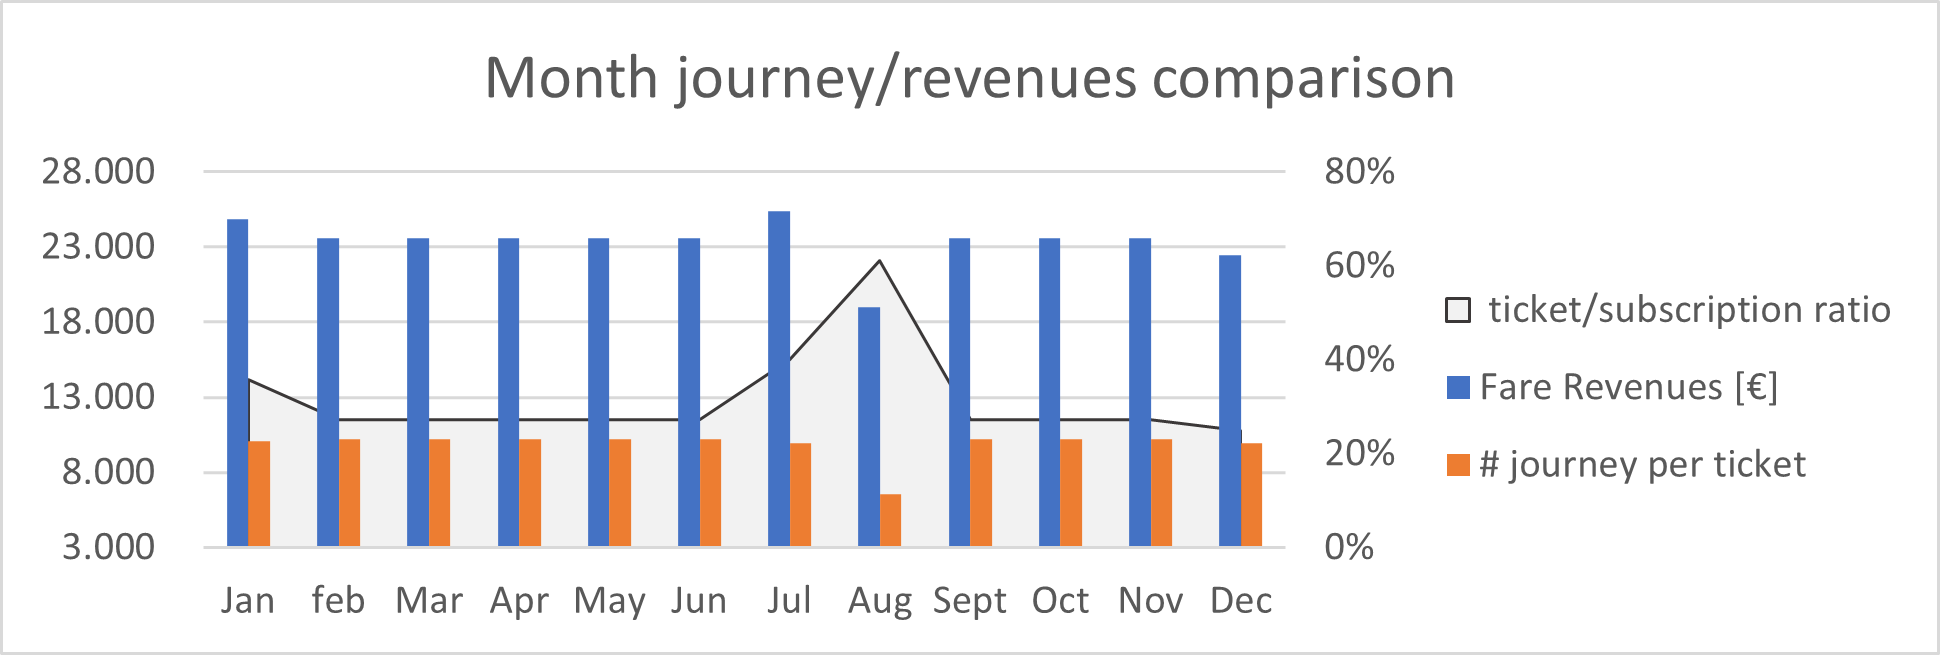
\includegraphics[width=0.7\textwidth]{Images/financial/journey_revenues.png}
    \caption{Journey Revenues}
    \label{fig:j_revenues}
\end{figure}

\section{Income statement}
Moving from the demand side to the offer one, the different economic performances of the two-service implementation scenario is analyzed. Their common feature are the distance between the depot and the service starting point (which accounts for 1.8 km) and the decision to avoid the usage of public subsidies, under the general idea to develop a self-sustainable business model.

\paragraph{scenario A}
Starting from the scenario A, it records an annual milage of 64 thousand of kilometers of which the 97\% in the economically productive “in service” state, and the remaining for the depo transfer. For more communicative data visualization, in figure \ref{fig:incstateA} are reported only major voices of the income statement.

\begin{figure}[h]
    \centering
    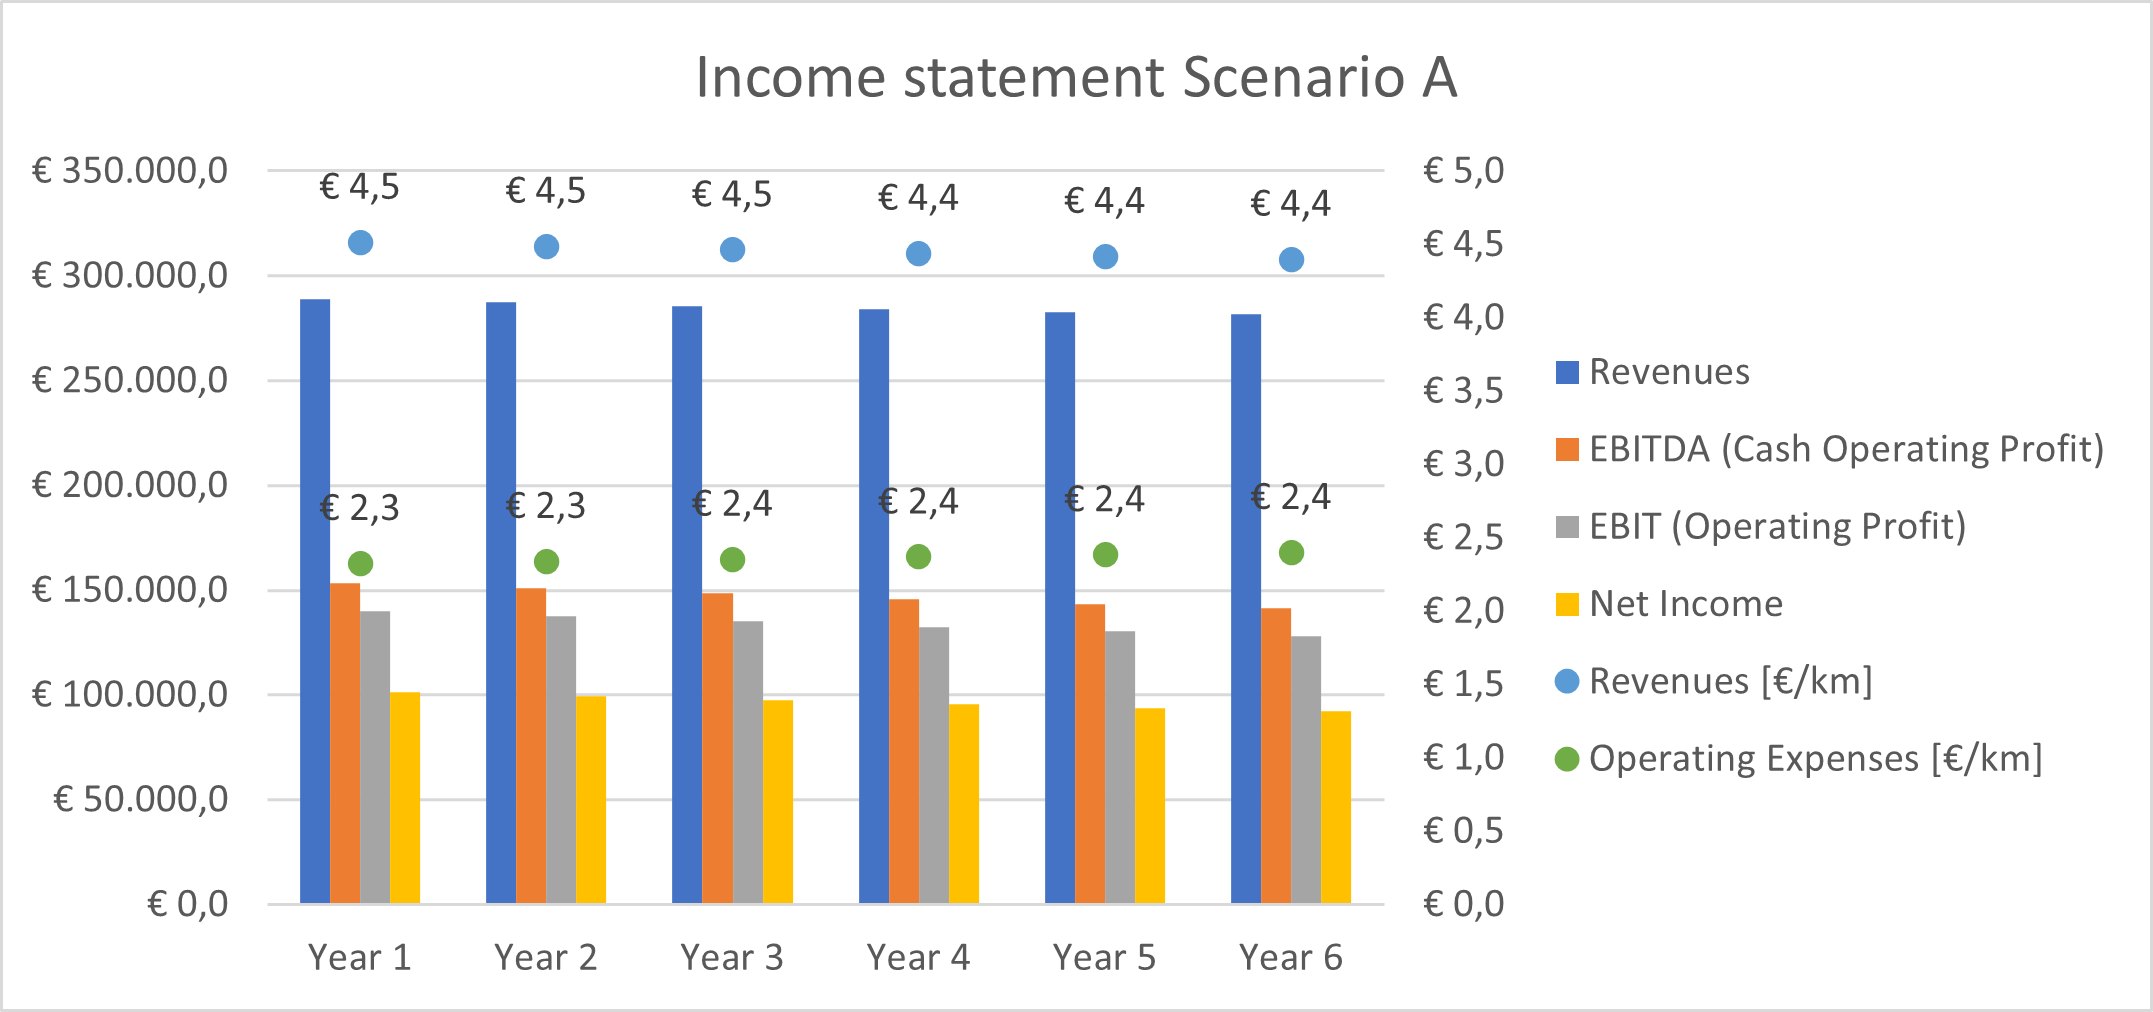
\includegraphics[width=0.7\textwidth]{Images/financial/income_statement_A.png}
    \caption{Scenario A: Income Statement}
    \label{fig:incstateA}
\end{figure}

Looking to the cost Structure, obtained by the “Cost of Goods and services” voice and showed in the pie chart below, it is noticed a slightly different composition respect to a traditional PTO cost structure, with an higher fuel cost incidence and a slightly less driver ones. 

\paragraph{scenario B}
Analyzing the second scenario, the B one, we have a small reduction in the annual performed milage (which accounts for 61.5 thousand annual kilometer, the 4\% less) with a consequent slightly higher incidence of the “Out of service” milage, which accounts for the 5\%. Nevertheless, despite these small variation, we almost have a coincidence in these previously values showing how the “hard” route deviation in the scenario B produce similar performances in the service implementation strategy with respect to the scenario A
The main Income statement voices related to this scenario are visualized in the \ref{fig:incstateB}.

\begin{figure}[h]
    \centering
    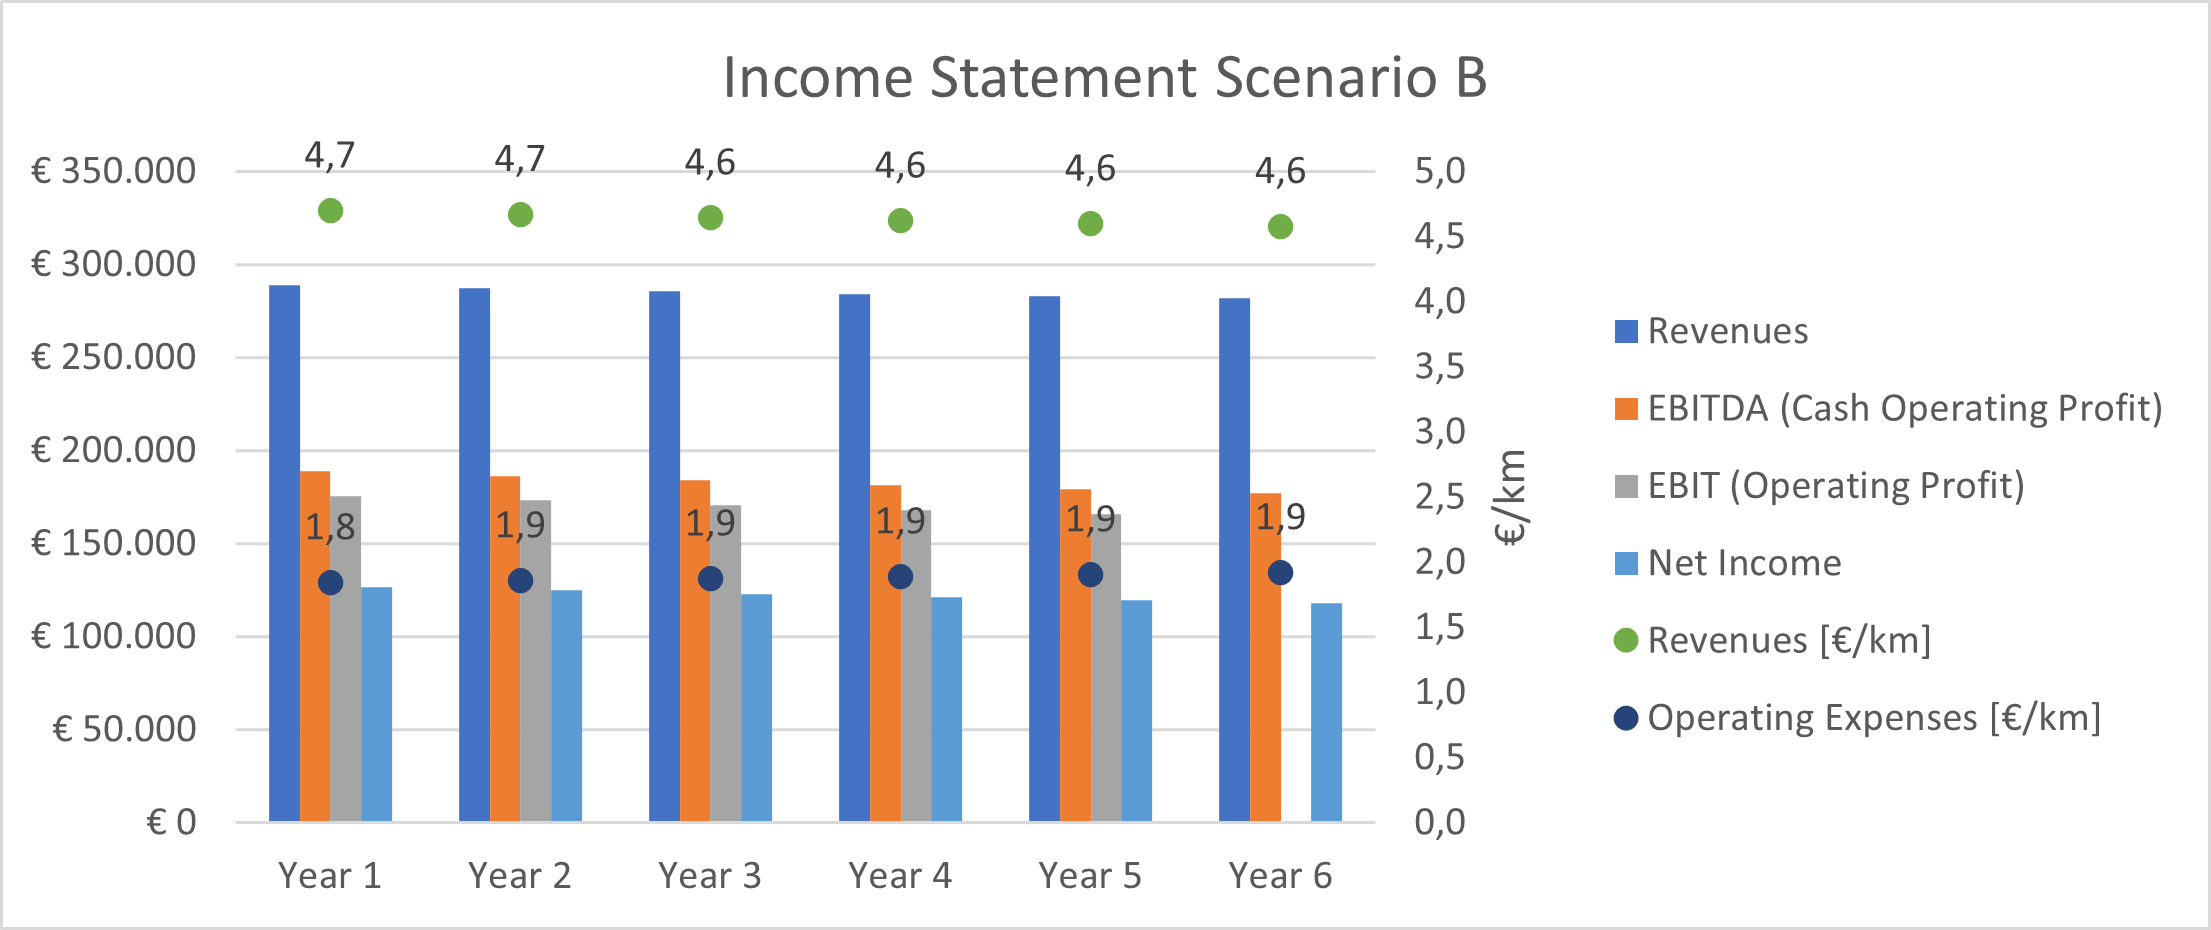
\includegraphics[width=0.7\textwidth]{Images/financial/income_statement_B.png}
    \caption{Scenario B: Income Statement}
    \label{fig:incstateB}
\end{figure}

\begin{figure}[h]
    \centering
    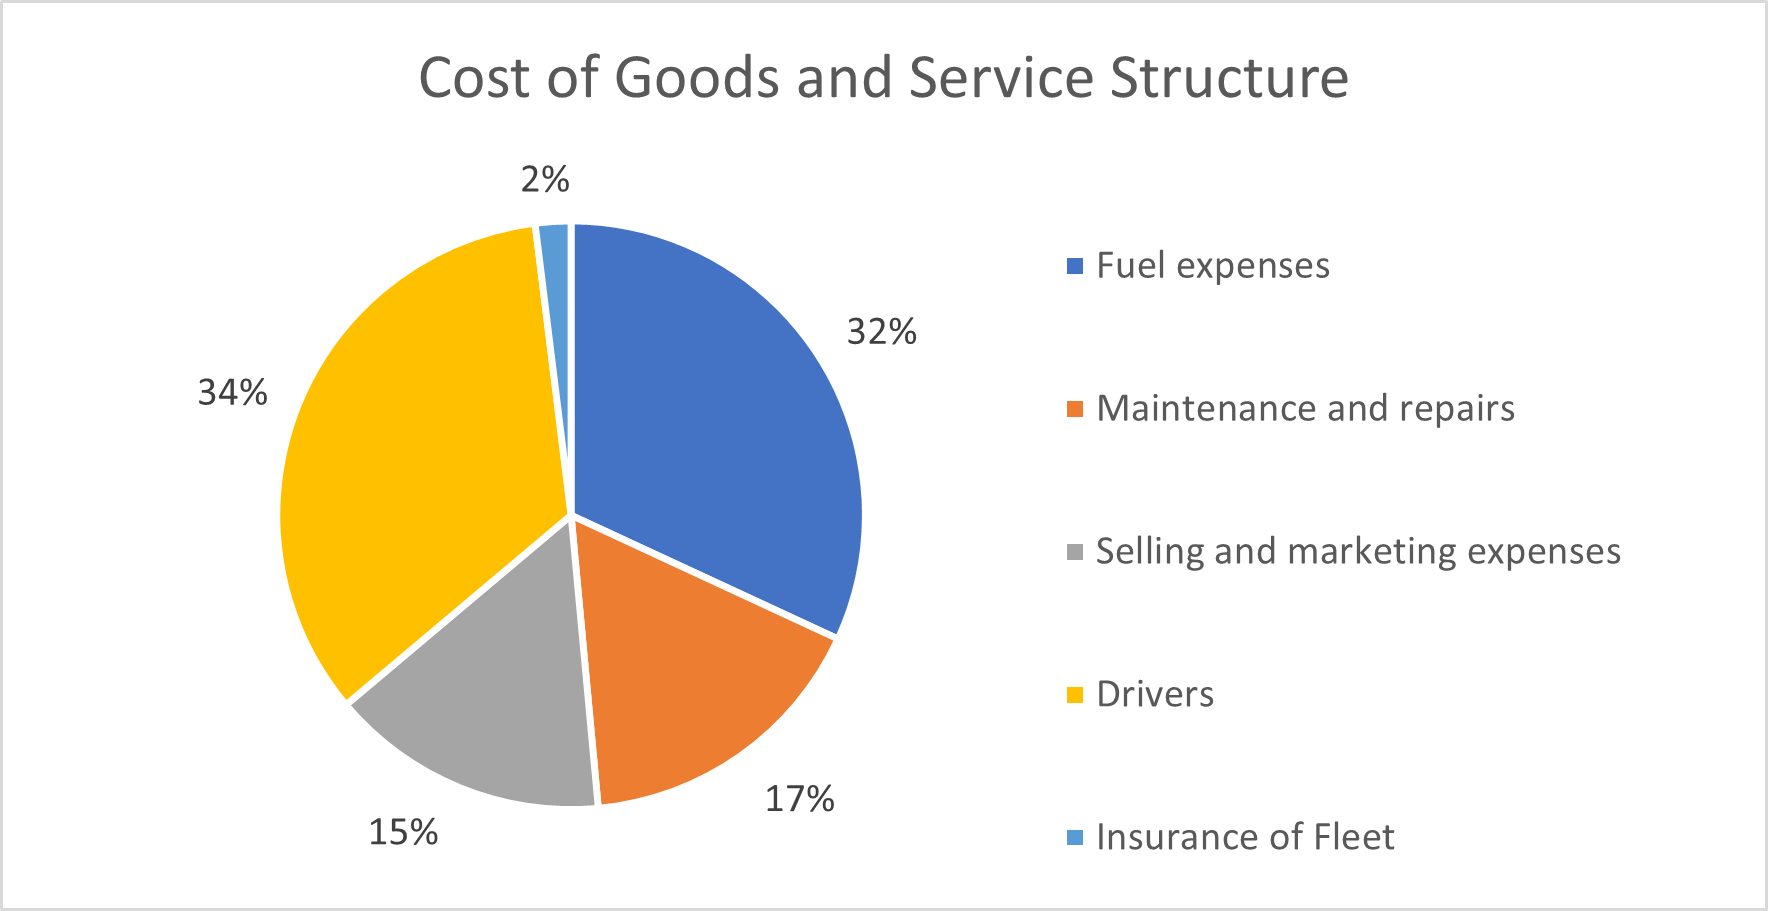
\includegraphics[width=0.7\textwidth]{Images/financial/Cost_of_Goods.png}
    \caption{Cost of Goods and Service Structure}
    \label{fig:costgoodsservice}
\end{figure}

\subsection{Income statement comparison}
Both the service scenarios scores more than acceptable economic performance all over the 6 studied year without the grants’ needs and without the effect of the progressively yearly revenues reduction.
The side-to-side comparison (reported in \ref{fig:income_statement_comparison}of the main income statement voices shows clearly how, from an economic perspective, the scenario B produce better economic performance. 

This phenomenon is simply due to the fewer operating cost of the B service (which perform less annual milage) and consequently by the higher ratio between revenues over distance – same revenue over a smaller distance. 

Consequently, given that the two scenarios produce the identical level of service for the customer, we agree to select the B scenario as best way for the company to implement the service in the most efficient way.

\begin{figure}[h]
    \centering
    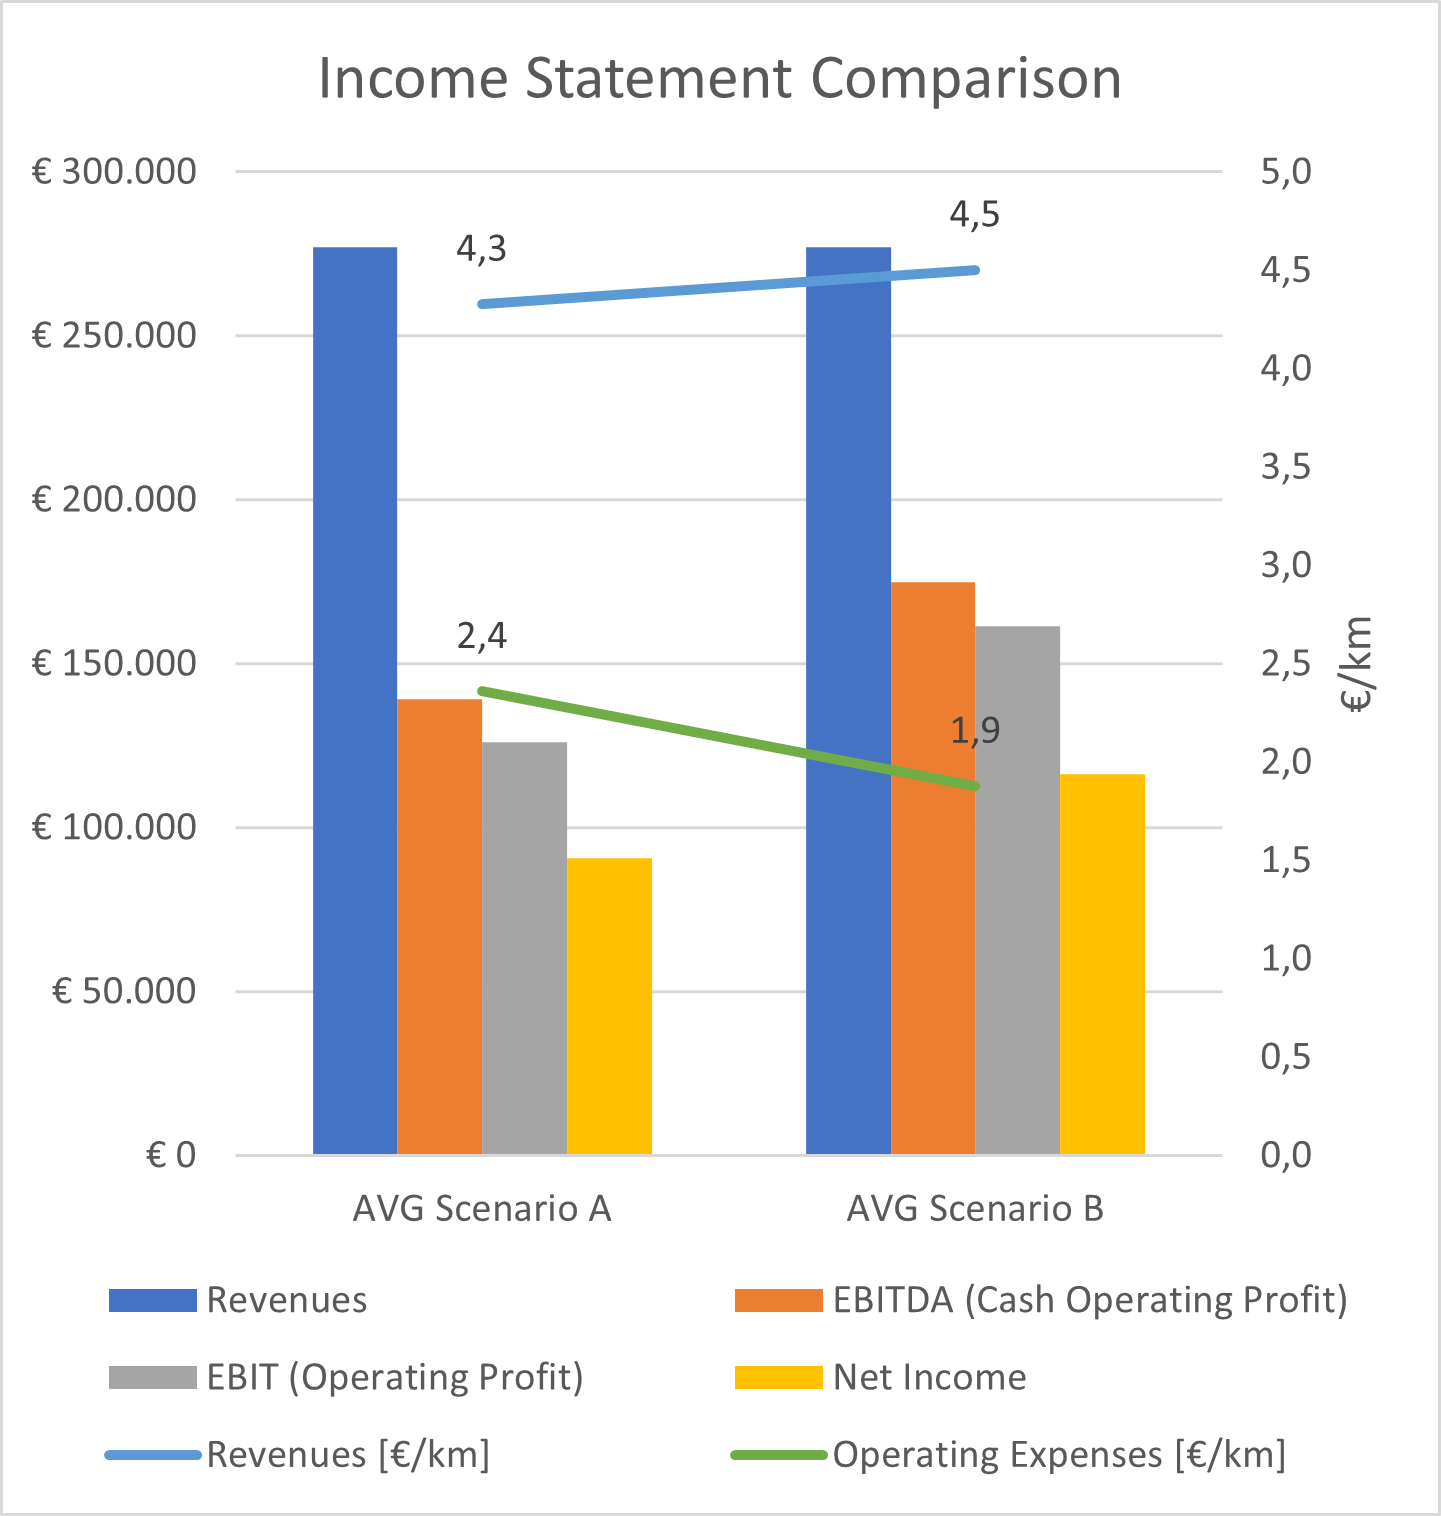
\includegraphics[width=0.7\textwidth]{Images/financial/Comparison.png}
    \caption{Income Statement Comparison}
    \label{fig:income_statement_comparison}
\end{figure}

\section{Sensitivity analysis}
This section will investigate the influence of some parameter’s variation, as “fuel cost” and the “passenger load”, over the economic performance. A cross analysis is performed to understand the combined power effect of the two above mentioned parameters, as a tool to understand the resilience of our business model to the last time world event (the higher passenger variability during the covid and after-covid period, combined with the energetic crisis due to the Ukraine war).

Because we select the hypothetical implementation of the scenario B, this analysis with be focused only on it.

The variability range used for the variables are:
\begin{itemize}
    \item +10\%, 0\%, - 10\% of the fuel cost
    \item +22\%, 0\%, -22\% of the mean passenger onboard (which means 34, 28, 22 travelling people)
\end{itemize}

On the offer side, the economic impact of the fuel cost variation described by the “Operating Cost”, is showed in the figure \ref{fig:opercost}.

\begin{figure}[h]
    \centering
    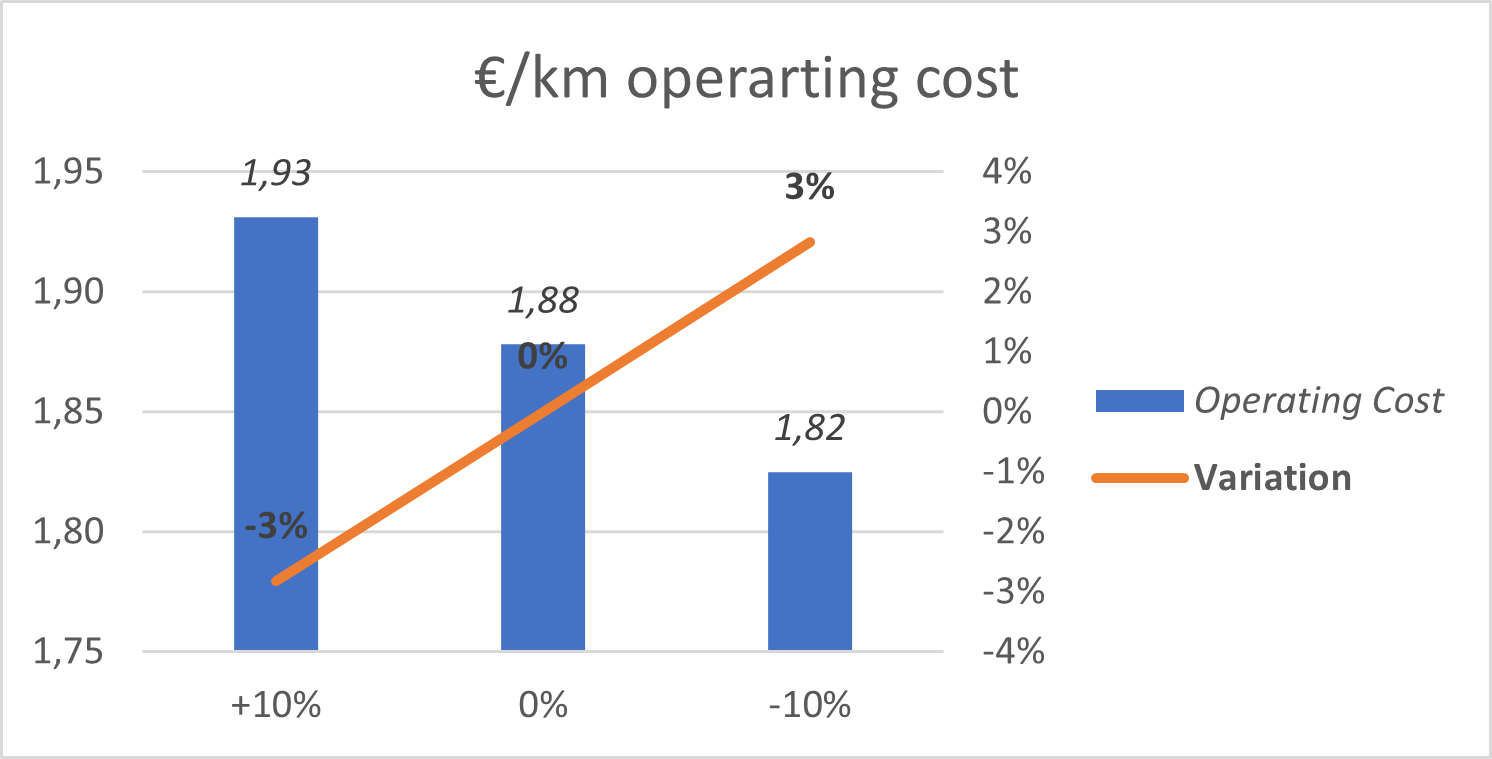
\includegraphics[width=0.7\textwidth]{Images/financial/operating_cost.png}
    \caption{Operating Cost}
    \label{fig:opercost}
\end{figure}

The consequent economic variation, in terms of “Delta EBIT” on percentage and distance metrics, is shown in figure \ref{fig:ebit},\ref{fig:ebitkm}.

\begin{figure}[h]
    \centering
    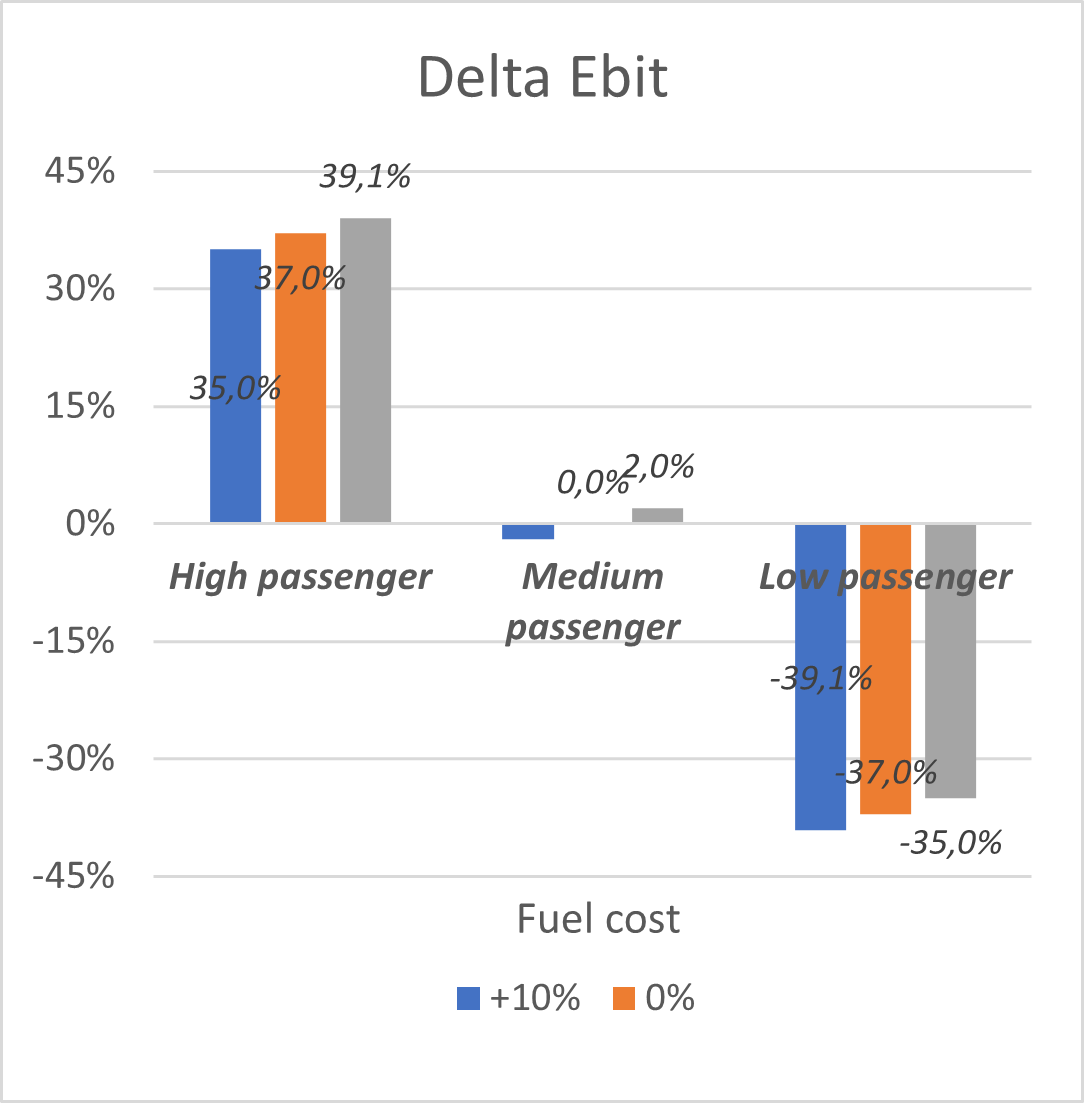
\includegraphics[width=0.7\textwidth]{Images/financial/ebitt.png}
    \caption{Delta EBIT}
    \label{fig:ebit}
\end{figure}

\begin{figure}[h]
    \centering
    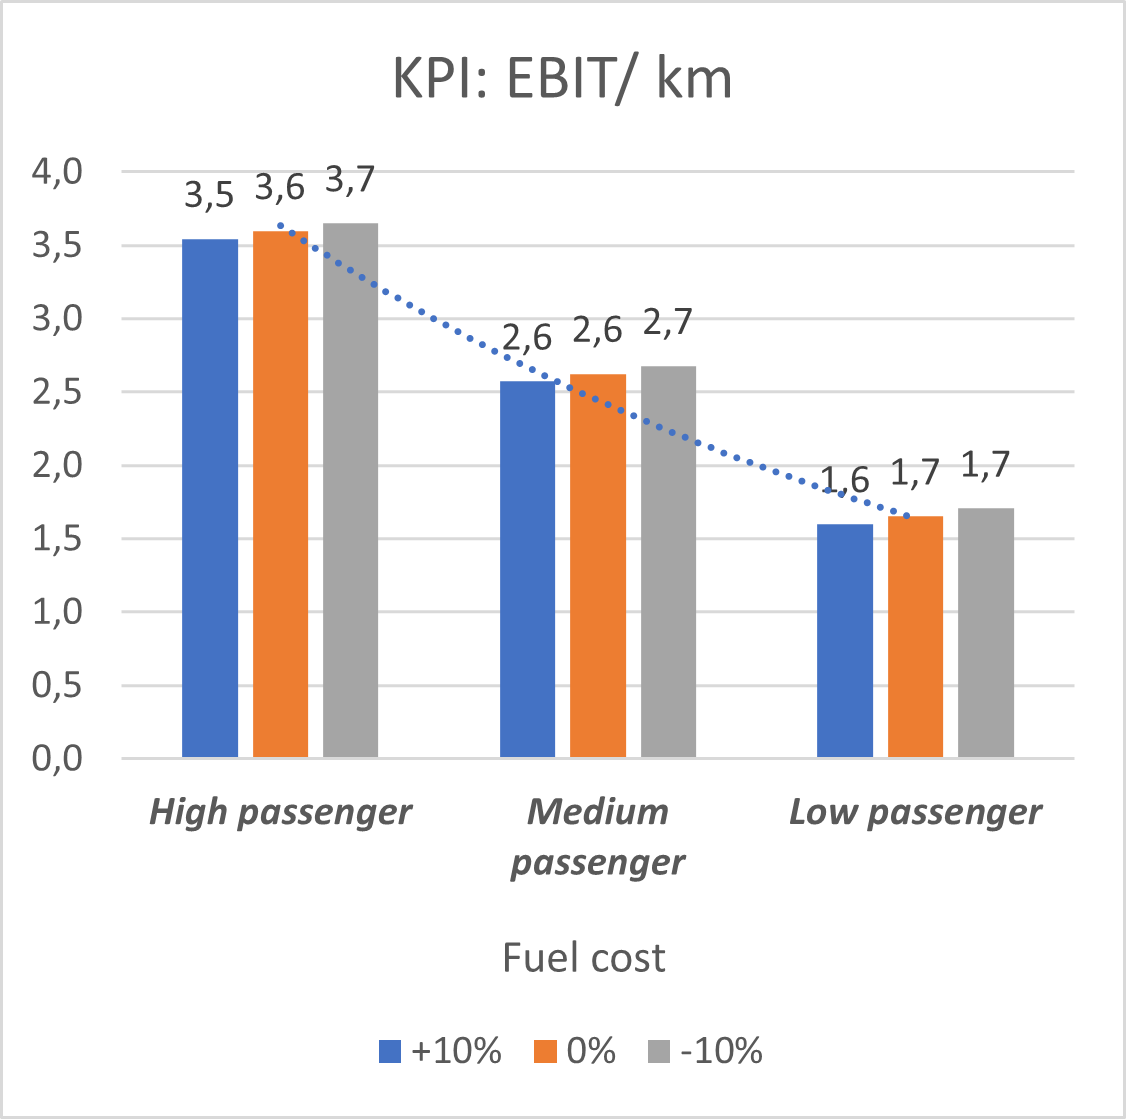
\includegraphics[width=0.7\textwidth]{Images/financial/ebitkm.png}
    \caption{EBIT/km}
    \label{fig:ebitkm}
\end{figure}

As is showed in these graphs, even in the “black-swan” scenario – increased fuel cost and the reduced number of passenger- our studied service is still able to generate cash from its operation, even if by 35\% less.

Lastly, give an average customer trip length of 33.2 km, even in the unrealistic case where all the on board passenger would be subscripted to seasonal ticket, the service would be still profitable, as represented in the table below.

